\chapter{Data collection}

%\section{The need for a dataset}
\section{Aims of a dataset}
The aims of collecting a dataset are to present a new set of recordings of a simple stimulus around which careful indepth analysis is possible. 
The dataset should emphasise the qualities the DVS has which standard cameras do not. 
In particular, motion information should be sought as datasets of inherently two dimensional stimuli (e.g. characters) already exist and make less sense as a processing task for the DVS.


%%%%%%%%%%%%%%%%%%%%%%%%%%       MOVED TO LIT REVIEW      %%%%%%%%%%%%%%%%%%%%%%%%%%%%%%%%%%%%%%%
%To fairly compare models it is necessary for the community to have standardised datasets\cite{barranco2016dataset, Gibson2014, tan2015benchmarking}.
%Many datasets exist for frame-based models from well formatted and normalised datasets (such as MNIST\cite{lecun1998gradient}) to large complex datasets (such as ImageNet\cite{deng2009imagenet}).
%In an attempt to compare event-based processing models to time-stepped models some have used DVS recordings of the classic MNIST dataset, being either with stationary images and a moving sensor \cite{OConnor2013, orchard2015converting} or with a sationary sensor and moving images on a screen \cite{serrano2015poker, akolkar2015can}.
%Notably different to others is the secondary digit dataset in \cite{akolkar2015can} in which a DVS performs vertical saccades while recording digits on a rotating cylinder.
%However in trying to be comparable with frame-based models these datasets fail to encompass the full potential of the DVS to capture complex spatio-temporal surfaces because the simulus is inherently two dimensional.
%Newer benchmark datasets have addressed this problem offering a wide range of stimuli, in particular complex real world self motion for a mobile robot \cite{Gibson2014, barranco2016dataset}. 
%Unfortunately there is still a deficency of extremely simple datasets around which strong mathmatical foundations can be laid to allow a deep understanding of network dynamics.
%Further as capturing movement is a key advantage of the DVS over frame-based sensors this should be emphasised in the dataset. 
%This work offers such a dataset consisting of dots moving linearly with constant velocity. 

\section{Requirements and details}
The motivations behind such a dataset must be carefully considered so when collected it forms a comprehensive set.
Simple structure is required so that the dynamics of a system can be accurately reasoned about when experimenting with new approaches to processing. 
%Simple structure is required so that when experimenting with new appraoches to processing dynamics in the system can be reasoned about with some accuracy.
Additionally datasets of complex real world (robotic self-motion etc.) already exists, it is simpler data that is missing.
To evaluate the accuracy of classification systems a ground truth is also required labelling events as signal or noise. 
The literature had many datasets classifying clusters of events, e.g. as a digit for MNIST or a direction for some of navigational datasets and as such work well for classification tasks.
For prediction tasks no per-event labelled dataset exists to allow simple calculations of model performance.  
The advent of deep learning has highlighted the advantages of large bodies of labeled training data. 
Thus the ability to collect a large number of samples is also deemed necessary and the system should be as autonomous as possible. \\ 
\textbf{Final requirements:}

\begin{itemize}
    \itemsep-0.5em
    \item \textbf{Simplicity} -- To allow model analysis
    \item \textbf{Movement} -- Key advantage of the DVS
    \item \textbf{Labels} -- To facilitate learning and validation
    \item \textbf{Autonomous} -- So large amounts can be captured
\end{itemize}

% TWO datasets 8AD and AAD
    % Each has several parameters; size, speed etc
    % Each combination of parameters has 1200 trials (150 per angle for 8AD) 


Considering the gap this dataset will fill and the requirements specified, the simplest stimuli was decided to be a single dot moving linearly with a constant velocity. 
The variables to be manipulated include the dot diameter, velocity and direction. 
These variations recorded are listed in table \ref{tb:datasetspecs}.

\begin{table}[h]
\centering
\begin{tabular}{ | c | l | }
    \hline
    Dot size (pixels) & 4, 6, 8 \\
    Angles (degrees) & [0 - 360] \\
    Starting position & Random \\
    Velocity (pixels/update) & 2, 4, 6, 8 \\
    \hline
\end{tabular}
\caption{Arbitrary Angle Dataset specification}
\label{tb:datasetspecs}
\end{table}

The above specification details what is from here on called the Arbitrary Angle Dataset (for brevity it will be referred to as AAD), that is, in this dataset the starting position of the dot does not restrict its direction.
An even simpler dataset from here on called the 8 Angle Dataset (for berevity, 8AD) is also presented in which the dot can only start from a corner of the screen or the middle of the one the edges.
The starting position of the dot also then dictates the direction the dot will move e.g. if it starts in the top left of the screen it must go to the bottom right or if it starts in the center of the top edge it must go to the center of the bottom edge.
Figure \ref{fig:8ADDirections} shows the directions used starting from each corner and edge center.

\begin{figure}
    \centering
    \includegraphics[width=0.4\textwidth]{8AD_directions.png}
    \caption{Directions allowed in 8AD}
    \label{fig:8ADDirections}
\end{figure}

As a stepping stone from simple datasets to more complex real world datasets two further variations were considered; two dots intersecting at the center of the screen and multiple dots tracing arbitrary angles (occasionally intersecting).
These additonal datasets are referred to as the Multiple Dot Datasets (MDD) from here. 





%%%%%%%%%%%%%%%%%%%%%%%%%%%%       CONSIDERATIONS    %%%%%%%%%%%%%%%%%%%%%%%%%%%%%%%%%
\section{Considerations}
\subsection{Stimulus generators}
With clear requirements the practical generation of the dataset can be considered in detail.
The requirement for constant velocity would prove difficult to control in any real world system with forces of friction and gravity.
Such a real world system would also prove uneconomical in terms of time required to construct and, unless well automated, time required to conduct recordings. 
Recording computer simulations becomes an attracive option (particularly in regards to recording ground truths) but comes with its own negatives including screen refresh rates.
Recording from a computer screen also brings the disadvantage of non-continuous stimuli, the dot must be discretised, drawn onto pixels and thus screen pixel size form the grid on which the stimuli is restricted. 
This issue can be mitigated when considering the much finer resolution of a screen compared to the DVS.
The discretisation of the dot on a screen will have minimal effect if the dot is comprised of enough screen pixels.
The non-continuous stimuli issue can likewise be alliviated by restricting the dot movement to low velocities meaning in any given refresh of the screen the dot only moves by a small amount and thus approximates continuous movement. 


\subsection{Data quality concerns}
%Flashes on screen -> noise
%Light invariance
%Ground truth to actual recording consideration (mitigated through setup?)

The DVS's temporal resolution of \SI{15}{\micro\second} means it should be able to detect screen refresh rates (every \SI{16}{\milli\second} on a 60Hz screen). 
It would be expected that every \SI{16}{\milli\second} there should be activity across the whole sensor for a short time period. 
%TODO come back and fix, opened backets and not closed.
This does not seem to be the case with the DVS; the same experiment run with the newer DAVIS sensor (with temporal resolution of \SI{3}{\micro\second} occasionally is able to capture the screen refresh rate but even this is not consistent as shown in figure \ref{fig:refreshFlashes}.


\begin{figure}
    \centering
    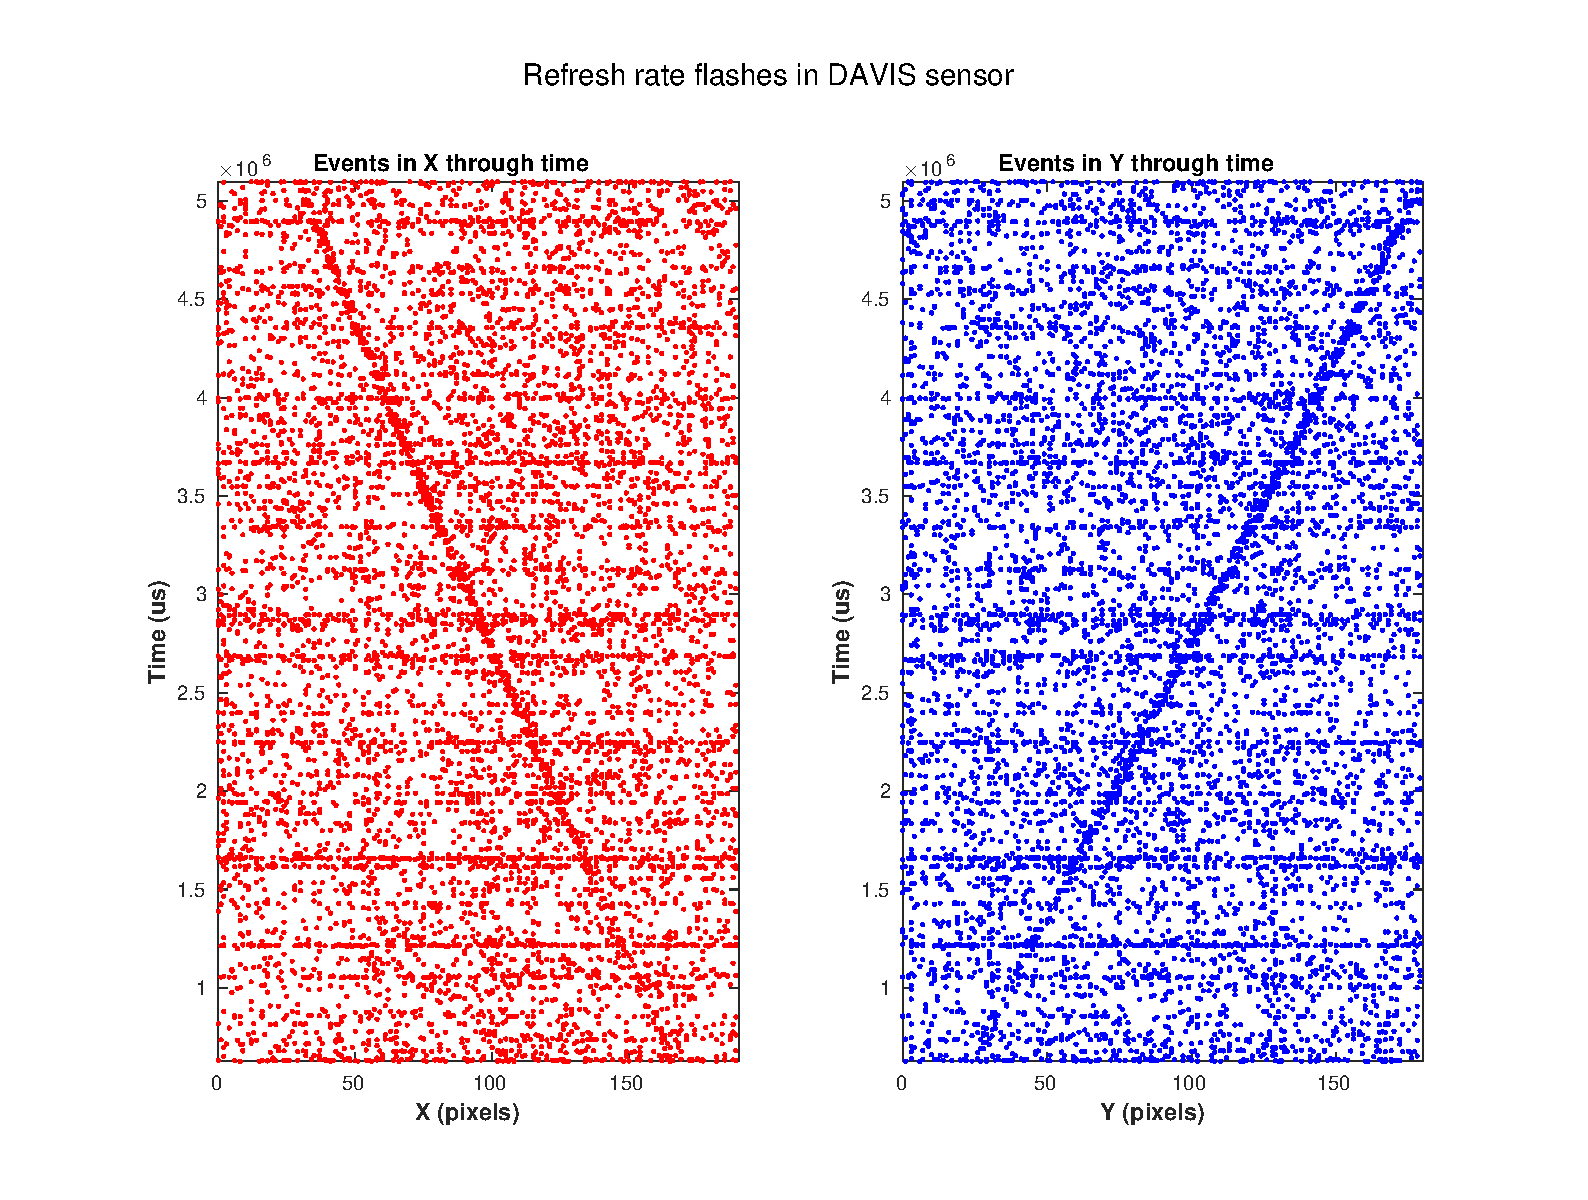
\includegraphics[width=0.8\textwidth]{screenFlashes.eps}
    \caption{Refresh rate flashes (horizontal lines) captured by DAVIS sensor}
    \label{fig:refreshFlashes}
\end{figure}

The DVS will only trigger an event if a pixels internal value has changed by 15\% meaning in low light situations the DVS will register an event more readily. 
Not all recording will be done in one session and changes to ambient light due to environmental conditions may have an impact on recording quality by triggering more or less events for the same stimuli.
In an effort to minimise this all recordings will be done on the same screen in a darkened lab and run overnight so there are no changes in ambient lighting. 

A more serious concern is that of ensuring label consistency between the screen pixels and the DVS pixels. 
When recording from the screen it will be critical to ensure the DVS is carefully aligned with the edges of the stimuli.
Failure to align the two will result in labels being misleading as the recording will be offset.
Lacking specialised equipment for a rigid recording aparatus and screen, this slight transformation of screen pixels to sensor pixels will become a characteristic of the datatset. 

\subsection{Processing considerations}
%Segmenting datasets
%Line angles (Close to edge, just a tiny segment in corner)
In an autonomous collection setup the question of data integrity must be raised.
Numerous situations could lead to the experimental setup becoming compromised without experimenter knowledge; such as the DVS being bumped.
Additionally, in processing the data computer ground truth labels may accumulate an offset after many trials.
These problems can be avoided by embedding meta-data in the data recordings which can be used to help keep processing synchronised and to validate the recording integrity. 
The meta-data to include was the trajectory of the line in the current trial as well as a horizontal and vertical line crossing at the center of the screen.
This will allow callibration of the DVS's rotational and linear offset from the center of the stimulus as well as tracking of the dot's path in this offset view. 
One trial in the dataset will be defined as a dot crossing from one edge of the screen to the other with its associated meta-data, thus a full trial will be:

\begin{itemize}
    \itemsep-0.5em
    \item Flash dot trajectory (30\ms)
    \item Actual sample (dot following trajectory)
    \item Flash dot trajectory (30\ms)
    \item Flash cross (30\ms)
    \item Repeat for the next trial
\end{itemize}

The process of flashing the dot trajectory, the cross and then the next dot's trajectory will be referred to as a meta-flash. 
Using these meta-flashes means the data can be independently verified and will produce a histogram of total number of spikes similar to figure \ref{fig:spikehistogram}.
This makes segmenting samples a matter of extracting the regions in which the total number of events is below some threshold (which varies proportionally to the size of the dot, and hence the number of events it produces). 

\begin{figure}
    \centering
    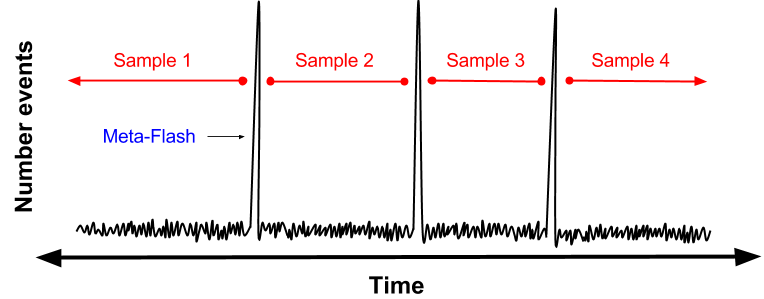
\includegraphics[width=0.8\textwidth]{metaflash.png}
    \caption{Histogram of the number of spikes during a recording}
    \label{fig:spikehistogram}
\end{figure}



In the arbitrary angle samples it will be possible for a dot to start close to a corner and to move to the adjacent edge resulting in a sample with a path of very few (\textless 5) DVS pixels and lasting less than a second.
This case was considered troublesome for later processing steps and thus the starting points in the arbitrary angle dataset were restricted to the middle 80\% of each edge. 

\subsection{DVS characteristics}
%Black on white and white on black, grey
%Hot pixels

The DVS is still a new research tool and as such still has some peculiarities, in particular due to the manufacturing process.
Some pixels, called 'hot pixels', in the array fire more frequently than others regardless of stimuli. 
These hot pixels are a source of noise in the data and could be removed in software or hardware but the effect is minimal compared with the standard noise of neuromorphic sensors so they were left in these experiments to avoid causing gaps in the input where there was no activity. 

DVS pixels will more readily fire if their internal value is smaller.
This has implications when the DVS is recording a black dot on a white screen or a white dot on a black screen.
The black screen means the DVS is more susceptible to ambient noise and will fire more events for a white dot, when compared to a black dot of the same size on a white screen. 
This phenomena is not expected to reveal any significant insight related to this thesis and is considered out of scope but its cause is worth considering whilst designing experiments. 



%%%%%%%%%%%%%%%%%%%%%%%%%%%          METHODOLOGY         %%%%%%%%%%%%%%%%%%%%%%%%%%%%%%
%TODO maybe this should just be a sub section since its so small, what else should go here?
\section{Method}
The datasets were collected automatically overnight by the python program dot\_gen. 
The dot\_gen software was custom made to present the stimulus on screen while logging the ground truth and interfacing with the jAER software package over UDP to start and stop recordings. 
The Tkinter software library was used for drawing the stimuli on screen. 
Experiments were run overnight to avoid any disturbances of general laboratory use during work hours as well as to mitigate ambient light changes for different times of day. 
A sample is defined as 1200 trials for a particular size and velocity pair for the dot.
On a given night either samples from the 8AD or AAD dataset were collected. 
By recording all parameters on all nights the noise between parameter combinations (due to computer screens in the lab or other ambient light changes) should remain somewhat uniform.

% TODO reference this figure somewhere
\begin{figure}
    \centering
    \includegraphics[width=0.7\textwidth]{DVS_dotgen.jpg}
    \caption{Experimental set up for recording datasets}
    \label{fig:DVSdotgen}
\end{figure}





% TODO this section mentions meta-flashes, should check they are explained above
%The final system consisted of a program called dot\_gen written in python which would display the dot moving along a trajectory with meta-flashes.
%The dot\_gen software also had tools to automatically start and stop DVS recordings, adjust dot parameters (size and velocity) and help set up the DVS correctly. 
%It would log the ground truth of the dots position to a CSV file in the format <x, y, time> every time the screen was updated.
%The screen recorded from was a Dell U2414H Monitor with a refresh rate of 60Hz.
% TODO Talk about the need for automation and overnight recordings
%Experiements were specified in the dot\_gen source code and were then run automatically overnight to avoid changes in ambient light.

\section{Per-event labels}
Ground truths for each recording are supplied with the data files however these only label where the dot was when the stimulus was updated and do not yet directly label the events.
Unification of the ground truth with the events recorded was not necessary for this work and due to time constraints has been excluded from the scope.
In this unification it may be important to consider small time differences between time zero in the ground truth log and the DVS recording.
This difference will be the time from when the dot\_gen software sets its time to zero, sends a UDP message to jAER and when jAER then sets its timestamp to zero. 
This communication all happened on a single machine and should be insignificant but may need to be considered. 
Further the unification process will require interpolation between the ground truths points which are sampled at the frequency of dot movement (~16\ms) and the event-data which is sampled roughly 10x more frequently.
The screen pixel to DVS pixel alignment may have an effect on the performance of such an algorithm. 
While care was taken to ensure the DVS captured just the stimulus screen, no metric to measure this mapping is defined and near perfect alignment between DVS pixels and screen pixels was not frequently achieved. 




%%%%%%%%%%%%%%%%%%%%%%%%%%%         FINAL SPECS          %%%%%%%%%%%%%%%%%%%%%%%%%%%%%%
\section{Discussion}
% TODO Fill in placeholders below
The final dataset submitted consists of ***EVENTS*** events from ***HOURS*** of recording split into ***NUMBER*** different files.
%This work offers a new datset consisting of simple linear motion for training and comparing models.
This work is a step towards filling the gap in current literature for a simple labelled motion-based dataset. 
Two main new datasets are presented featuring linear motion with constant velocity along 8 Angles or Arbitrary Angles.
These datasets fill the requirements of being simple, motion based, labelled and simple to collect automatically.
Some concerns for data quality remain as to whether refresh rates are noticeable in the dataset and whether the slight transformations between DVS pixels and screen pixels will affect the per-event labelling accuracy.
By embedding meta-flashes directly in the data some degree of calibration in the labels can be maintained along with the ground truth logs. 
Further work is required to unify the ground truth logs with the recordings to generate labelled events but is considered out of scope for this work which will process the data differently. 

% TODO this section feels a little disjoint -> need to clarify the sections/points I am trying to make
% Problems with SCREen PIXEL TO DVS PIXEL line up
%   Which ties into general DVS position -> edges not perfect
% Further processing of ground truth events labels required and not considered here

% MOVE TO PROCESSING - Segmenting looses a lot on each side \hfill
%No metric for validating ground truth against actual dot accuracy
